% !TeX program = xelatex
\documentclass{article}
\usepackage{kotex}
\usepackage[a4paper,left=3cm, right=3cm, top=2cm, bottom=2cm]{geometry}
\usepackage{amsmath}
\usepackage{graphicx}
\usepackage{caption}
\usepackage{setspace}
\usepackage{xcolor}
\usepackage{titlesec}
\usepackage{amssymb}
\usepackage{tcolorbox}
\usepackage{amsthm}
\usepackage{multirow}
\usepackage{array}
\usepackage{booktabs}
\usepackage{tikz}
\usetikzlibrary{positioning,arrows.meta,calc,shapes.geometric}
\usepackage{pgfplots}
\pgfplotsset{compat=1.18}

\title{8.2 Compositions and Inverse Transformations}
\date{}
\author{}
\setstretch{1.3}

\titleformat{name=\section, numberless}
  {\normalfont\large\bfseries\color{blue}}{}
  {0pt}{}
\geometry{a4paper, margin=1in}

\newcommand{\redheading}[1]{{\vspace{2mm}\noindent\Large\bfseries\color{red!55!black} #1\par}\vspace{2mm}}

\begin{document}
\maketitle

{\itshape\color{blue!45!black}
In Section~1.9 we discussed compositions and inverses of matrix transformations. In this
section we extend those ideas to general linear transformations.\par}

\vspace{2mm}

\redheading{One-to-One and Onto}

\begin{tcolorbox}[colback=teal!4, colframe=teal!65!black,
  title={\textbf{Definition 1}}, boxrule=0.5mm, arc=3mm]
If $T : V \to W$ is a linear transformation, then $T$ is \textbf{one-to-one} if $T$
maps distinct vectors in $V$ into distinct vectors in $W$.
\end{tcolorbox}

\begin{tcolorbox}[colback=teal!4, colframe=teal!65!black,
  title={\textbf{Definition 2}}, boxrule=0.5mm, arc=3mm]
If $T : V \to W$ is a linear transformation, then $T$ is \textbf{onto} (or \textbf{onto}
$W$) if every vector in $W$ is the image of at least one vector in $V$.
\end{tcolorbox}

\begin{figure}[ht]
\centering
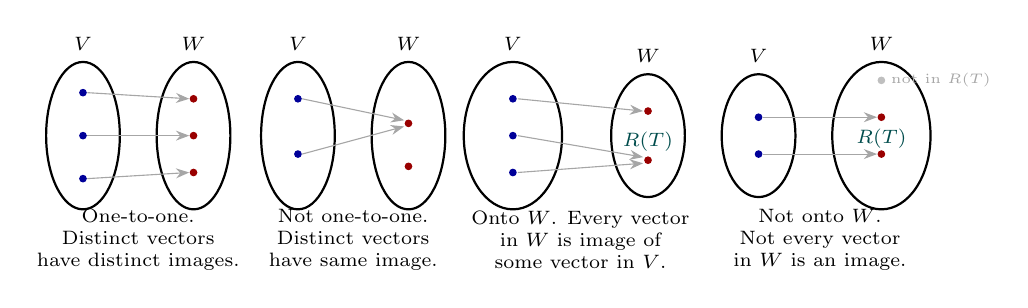
\begin{tikzpicture}[>=Stealth, scale=0.78]
  % Panel 1: One-to-one
  \begin{scope}[xshift=0cm]
    \draw[thick] (0,0) ellipse (0.6 and 1.2);
    \draw[thick] (1.8,0) ellipse (0.6 and 1.2);
    \node[font=\scriptsize] at (0,1.5) {$V$};
    \node[font=\scriptsize] at (1.8,1.5) {$W$};
    \foreach \y/\dy in {0.7/0.6, 0/0, -0.7/-0.6}{
      \filldraw[blue!60!black] (0,\y) circle (1.5pt);
      \filldraw[red!60!black] (1.8,\dy) circle (1.5pt);
      \draw[->, gray!70] (0.07,\y) -- (1.73,\dy);
    }
    \node[font=\scriptsize, align=center] at (0.9,-1.7)
      {One-to-one.\\Distinct vectors\\have distinct images.};
  \end{scope}
  % Panel 2: Not one-to-one
  \begin{scope}[xshift=3.5cm]
    \draw[thick] (0,0) ellipse (0.6 and 1.2);
    \draw[thick] (1.8,0) ellipse (0.6 and 1.2);
    \node[font=\scriptsize] at (0,1.5) {$V$};
    \node[font=\scriptsize] at (1.8,1.5) {$W$};
    \filldraw[blue!60!black] (0,0.6) circle (1.5pt);
    \filldraw[blue!60!black] (0,-0.3) circle (1.5pt);
    \filldraw[red!60!black] (1.8,0.2) circle (1.5pt);
    \filldraw[red!60!black] (1.8,-0.5) circle (1.5pt);
    \draw[->, gray!70] (0.07,0.6) -- (1.73,0.25);
    \draw[->, gray!70] (0.07,-0.3) -- (1.73,0.15);
    \node[font=\scriptsize, align=center] at (0.9,-1.7)
      {Not one-to-one.\\Distinct vectors\\have same image.};
  \end{scope}
  % Panel 3: Onto
  \begin{scope}[xshift=7.0cm]
    \draw[thick] (0,0) ellipse (0.8 and 1.2);
    \draw[thick] (2.2,0) ellipse (0.6 and 1.0);
    \node[font=\scriptsize] at (0,1.5) {$V$};
    \node[font=\scriptsize] at (2.2,1.3) {$W$};
    \filldraw[blue!60!black] (0,0.6) circle (1.5pt);
    \filldraw[blue!60!black] (0,0) circle (1.5pt);
    \filldraw[blue!60!black] (0,-0.6) circle (1.5pt);
    \filldraw[red!60!black] (2.2,0.4) circle (1.5pt);
    \filldraw[red!60!black] (2.2,-0.4) circle (1.5pt);
    \draw[->, gray!70] (0.08,0.6) -- (2.12,0.4);
    \draw[->, gray!70] (0.08,0) -- (2.12,-0.35);
    \draw[->, gray!70] (0.08,-0.6) -- (2.12,-0.45);
    \node[font=\scriptsize, teal!60!black] at (2.2,-0.1) {$R(T)$};
    \node[font=\scriptsize, align=center] at (1.1,-1.7)
      {Onto $W$. Every vector\\in $W$ is image of\\some vector in $V$.};
  \end{scope}
  % Panel 4: Not onto
  \begin{scope}[xshift=11.0cm]
    \draw[thick] (0,0) ellipse (0.6 and 1.0);
    \draw[thick] (2.0,0) ellipse (0.8 and 1.2);
    \node[font=\scriptsize] at (0,1.3) {$V$};
    \node[font=\scriptsize] at (2.0,1.5) {$W$};
    \filldraw[blue!60!black] (0,0.3) circle (1.5pt);
    \filldraw[blue!60!black] (0,-0.3) circle (1.5pt);
    \filldraw[red!60!black] (2.0,0.3) circle (1.5pt);
    \filldraw[red!60!black] (2.0,-0.3) circle (1.5pt);
    \filldraw[gray!50] (2.0,0.9) circle (1.5pt)
      node[right, font=\tiny, gray!70]{not in $R(T)$};
    \draw[->, gray!70] (0.07,0.3) -- (1.93,0.3);
    \draw[->, gray!70] (0.07,-0.3) -- (1.93,-0.3);
    \node[font=\scriptsize, teal!60!black] at (2.0,-0.05) {$R(T)$};
    \node[font=\scriptsize, align=center] at (1.0,-1.7)
      {Not onto $W$.\\Not every vector\\in $W$ is an image.};
  \end{scope}
\end{tikzpicture}
\caption*{FIGURE 8.2.1}
\end{figure}

The one-to-one property can also be expressed as:
\begin{enumerate}
  \item[1.] $T : V \to W$ is one-to-one if and only if for each $\mathbf{w}$ in the range
  of $T$ there is exactly one $\mathbf{v}$ in $V$ with $T(\mathbf{v}) = \mathbf{w}$.
  \item[2.] $T : V \to W$ is one-to-one if and only if $T(\mathbf{u}) = T(\mathbf{v})$
  implies $\mathbf{u} = \mathbf{v}$.
\end{enumerate}

\begin{tcolorbox}[colback=red!4, colframe=red!60!black,
  title={\textbf{Theorem 8.2.1}}, boxrule=0.5mm, arc=3mm]
If $T : V \to W$ is a linear transformation, the following are equivalent:
\begin{enumerate}
  \item[(a)] $T$ is one-to-one.
  \item[(b)] $\ker(T) = \{\mathbf{0}\}$.
\end{enumerate}
\end{tcolorbox}

\textbf{Proof $(a)\Rightarrow(b)$.} Since $T$ is linear, $T(\mathbf{0}) = \mathbf{0}$.
Since $T$ is one-to-one, no other vector maps to $\mathbf{0}$, so $\ker(T) = \{\mathbf{0}\}$.

\textbf{Proof $(b)\Rightarrow(a)$.} Suppose $\ker(T) = \{\mathbf{0}\}$ and $\mathbf{u},\mathbf{v}$
are distinct vectors in $V$, so $\mathbf{u}-\mathbf{v} \neq \mathbf{0}$. If $T(\mathbf{u}-\mathbf{v})
= \mathbf{0}$, then $\mathbf{u}-\mathbf{v}$ would be in $\ker(T)$, a contradiction. So
$T(\mathbf{u}) - T(\mathbf{v}) = T(\mathbf{u}-\mathbf{v}) \neq \mathbf{0}$, meaning $T$ is
one-to-one. $\blacksquare$

\subsection*{EXAMPLE 1 | Rotation Operators on $R^2$ Are One-to-One and Onto}

The linear operator $T : R^2 \to R^2$ rotating each vector through angle $\theta$ is
one-to-one: distinct vectors rotate into distinct vectors (Figure~8.2.2). It is also onto
because every vector in $R^2$ is a rotation of another vector through $\theta$.

\begin{figure}[ht]
\centering
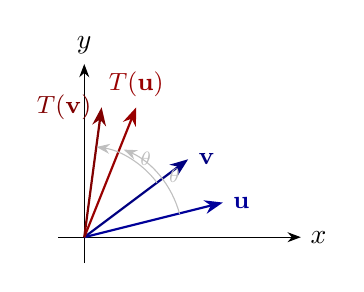
\begin{tikzpicture}[>=Stealth, scale=1.1]
  \draw[->] (-0.3,0)--(2.5,0) node[right]{$x$};
  \draw[->] (0,-0.3)--(0,2.0) node[above]{$y$};
  \draw[->, thick, blue!60!black] (0,0)--(1.6,0.4) node[right, font=\small]{$\mathbf{u}$};
  \draw[->, thick, blue!50!black] (0,0)--(1.2,0.9) node[right, font=\small]{$\mathbf{v}$};
  \draw[->, thick, red!60!black] (0,0)--(0.6,1.5) node[above, font=\small]{$T(\mathbf{u})$};
  \draw[->, thick, red!50!black] (0,0)--(0.2,1.5) node[left, font=\small]{$T(\mathbf{v})$};
  \draw[gray!50, ->] (1.1,0.27) arc[start angle=15, end angle=67, radius=1.12]
    node[midway, right, font=\scriptsize]{$\theta$};
  \draw[gray!50, ->] (0.84,0.63) arc[start angle=37, end angle=82, radius=1.06]
    node[midway, right, font=\scriptsize]{$\theta$};
\end{tikzpicture}
\caption*{FIGURE 8.2.2\quad Distinct vectors $\mathbf{u}$ and $\mathbf{v}$ rotate into distinct
vectors $T(\mathbf{u})$ and $T(\mathbf{v})$.}
\end{figure}

\subsection*{EXAMPLE 2 | Orthogonal Projections in $R^2$ Are Not One-to-One}

The operator $T : R^2 \to R^2$ projecting onto the $x$-axis maps distinct points on any
vertical line to the same point on the $x$-axis, so it is not one-to-one (Figure~8.2.3).
It is also not onto because points off the $x$-axis are not images.

\begin{figure}[ht]
\centering
\begin{tikzpicture}[>=Stealth, scale=1.0]
  \draw[->] (-1.5,0)--(2.5,0) node[right]{$x$};
  \draw[->] (0,-0.3)--(0,2.0) node[above]{$y$};
  \filldraw[blue!60!black] (1,1.5) circle (2pt) node[right, font=\small]{$P$};
  \filldraw[blue!60!black] (1,0.6) circle (2pt) node[right, font=\small]{$Q$};
  \filldraw[red!60!black] (1,0) circle (2pt) node[below, font=\small]{$M$};
  \draw[->, gray!60, dashed] (1,1.5)--(1,0.05);
  \draw[->, gray!60, dashed] (1,0.6)--(1,0.05);
\end{tikzpicture}
\caption*{FIGURE 8.2.3\quad Distinct points $P$ and $Q$ both project to $M$.}
\end{figure}

\subsection*{EXAMPLE 3 | Two Transformations That Are One-to-One and Onto}

$T_1 : P_3 \to R^4$ and $T_2 : M_{22} \to R^4$ defined by
\[
  T_1(a+bx+cx^2+dx^3) = (a,b,c,d) \qquad
  T_2\!\left(\begin{bmatrix}a&b\\c&d\end{bmatrix}\right) = (a,b,c,d)
\]
are both onto $R^4$ (any $(a,b,c,d)$ is achievable) and one-to-one (kernels contain only
$\mathbf{0}$—verify).

\subsection*{EXAMPLE 4 | A One-to-One Transformation That Is Not Onto}

The transformation $T : P_n \to P_{n+1}$, $T(\mathbf{p}) = xp(x)$ from Example~5 of
Section~8.1 is one-to-one: if $p(x) \neq q(x)$ they differ in some coefficient, so
$T(\mathbf{p}) = xp(x)$ and $T(\mathbf{q}) = xq(x)$ also differ. However, $T$ is not onto
because no polynomial in $P_n$ maps to the constant polynomial $1 \in P_{n+1}$ (every
image has a zero constant term).

\subsection*{EXAMPLE 5 | Shifting Operators}

Let $V = R^\infty$ be the sequence space and define the shifting operators
\[
  T_1(u_1,u_2,\ldots,u_n,\ldots) = (0,u_1,u_2,\ldots,u_n,\ldots)
\]
\[
  T_2(u_1,u_2,\ldots,u_n,\ldots) = (u_2,u_3,\ldots,u_n,\ldots)
\]
\textbf{(a)} $T_1$ is one-to-one: distinct sequences have distinct images (distinct entries
are just shifted). It is not onto: no vector maps to $(1,0,0,\ldots)$.

\textbf{(b)} $T_2$ is onto: any sequence $(u_2,u_3,\ldots)$ is the image of $(0,u_2,u_3,\ldots)$.
It is not one-to-one: both $(1,0,0,\ldots)$ and $(2,0,0,\ldots)$ map to $(0,0,\ldots)$.

\subsection*{EXAMPLE 6 | Differentiation Is Not One-to-One}
\textit{(Calculus Required)}

The differentiation operator $D : C^1(-\infty,\infty) \to F(-\infty,\infty)$, $D(\mathbf{f}) = f'(x)$,
is not one-to-one because functions differing by a constant have the same derivative:
$D(x^2) = D(x^2+1) = 2x$.

When $V$ and $W$ are finite-dimensional with equal dimension, a third condition can be added
to Theorem~8.2.1.

\begin{tcolorbox}[colback=red!4, colframe=red!60!black,
  title={\textbf{Theorem 8.2.2}}, boxrule=0.5mm, arc=3mm]
If $V$ and $W$ are finite-dimensional vector spaces with $\dim(V)=\dim(W)$, and
$T : V \to W$ is a linear transformation, the following are equivalent:
\begin{enumerate}
  \item[(a)] $T$ is one-to-one.
  \item[(b)] $\ker(T) = \{\mathbf{0}\}$.
  \item[(c)] $T$ is onto $[R(T) = W]$.
\end{enumerate}
\end{tcolorbox}

\textit{Proof.} Parts (a) and (b) are equivalent by Theorem~8.2.1. The equivalence of
(b) and (c) follows by applying Theorem~8.1.4 with $\dim(V)=n$: since
$\text{rank}(T)+\text{nullity}(T) = n$, we have $\text{nullity}(T)=0$ if and only if
$\text{rank}(T)=n = \dim(W)$, which means $R(T) = W$. $\blacksquare$

\textit{Remark on dimension.} If $\dim(W) < \dim(V)$, then $T$ cannot be one-to-one.
If $\dim(V) < \dim(W)$, then $T$ cannot be onto.

\vspace{2mm}

\redheading{Matrix Transformations Revisited}

\subsection*{EXAMPLE 7 | Matrix Transformations from $R^n$ to $R^m$}

If $T_A : R^n \to R^m$ is multiplication by an $m\times n$ matrix $A$:
\begin{itemize}
  \item If $m < n$: $T_A$ is not one-to-one (nullity $> 0$) and may or may not be onto.
  \item If $n < m$: $T_A$ is not onto and may or may not be one-to-one.
  \item If $m = n$: whether $T_A$ is one-to-one/onto depends on the rank of $A$.
\end{itemize}
If $A$ is invertible, $T_A$ is both one-to-one and onto.

\begin{tcolorbox}[colback=red!4, colframe=red!60!black,
  title={\textbf{Theorem 8.2.3}}, boxrule=0.5mm, arc=3mm]
If $T_A : R^n \to R^m$ is a matrix transformation, then:
\begin{enumerate}
  \item[(a)] $T_A$ is one-to-one if and only if the columns of $A$ are linearly independent.
  \item[(b)] $T_A$ is onto if and only if the columns of $A$ span $R^m$.
\end{enumerate}
\end{tcolorbox}

\textbf{Proof of (a).} By Theorem~8.2.1, $T_A$ is one-to-one iff $\ker(T_A) = \{\mathbf{0}\}$,
i.e., $A$ has nullity 0. By Theorem~4.9.2, this means $A$ has rank $m$ columns being
linearly independent (full column rank).

\textbf{Proof of (b).} $T_A$ is onto iff $R(T_A) = R^m$, i.e., every $\mathbf{b} \in R^m$
lies in the column space of $A$ (Theorem~4.8.1). $\blacksquare$

\begin{tcolorbox}[colback=red!4, colframe=red!60!black,
  title={\textbf{Theorem 8.2.4 --- Equivalent Statements}}, boxrule=0.5mm, arc=3mm]
If $A$ is an $n\times n$ matrix, the following are equivalent (adding to the prior
equivalence list):
\begin{enumerate}
  \item[(a)] $A$ is invertible.
  \item[(b)] $A\mathbf{x} = \mathbf{0}$ has only the trivial solution.
  \item[(c)] The reduced row echelon form of $A$ is $I_n$.
  \item[(d)] $A$ is a product of elementary matrices.
  \item[(e)] $A\mathbf{x} = \mathbf{b}$ is consistent for every $n\times 1$ matrix $\mathbf{b}$.
  \item[(f)] $A\mathbf{x} = \mathbf{b}$ has exactly one solution for every $n\times 1$ matrix $\mathbf{b}$.
  \item[(g)] $\det(A) \neq 0$.
  \item[(h)] The column vectors of $A$ are linearly independent.
  \item[\ldots]
  \item[(t)] The kernel of $T_A$ is $\{\mathbf{0}\}$.
  \item[(u)] The range of $T_A$ is $R^n$.
  \item[(v)] $T_A$ is one-to-one.
\end{enumerate}
\end{tcolorbox}

The same subspace of $R^n$ can be viewed three ways:
\begin{itemize}
  \item \textbf{Matrix view:} null space of $A$
  \item \textbf{System view:} solution space of $A\mathbf{x}=\mathbf{0}$
  \item \textbf{Transformation view:} kernel of $T_A$
\end{itemize}
Similarly the same subspace of $R^m$ can be viewed as the column space, the set of consistent
right-hand sides, or the range of $T_A$.

\vspace{2mm}

\redheading{Inverse Linear Transformations}

If $T : V \to W$ is one-to-one and $\mathbf{w}$ is any vector in $R(T)$, there is exactly
one $\mathbf{v}$ in $V$ with $T(\mathbf{v}) = \mathbf{w}$. This defines the \textbf{inverse}
$T^{-1} : R(T) \to V$ by $T^{-1}(\mathbf{w}) = \mathbf{v}$.

\begin{figure}[ht]
\centering
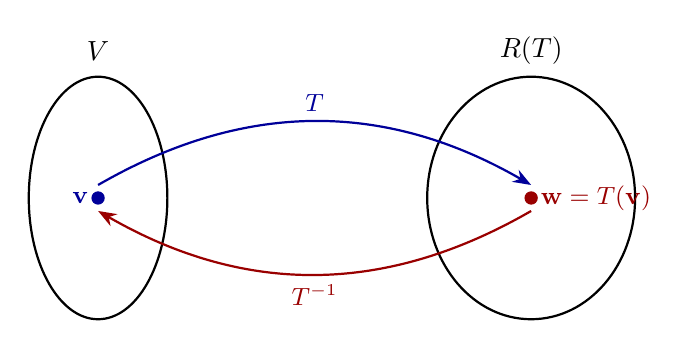
\begin{tikzpicture}[>=Stealth, scale=1.1]
  \draw[thick] (-2.5,0) ellipse (0.8 and 1.4);
  \node at (-2.5,1.7) {$V$};
  \draw[thick] (2.5,0) ellipse (1.2 and 1.4);
  \node at (2.5,1.7) {$R(T)$};
  \filldraw[blue!60!black] (-2.5,0) circle (2pt) node[left, font=\small]{$\mathbf{v}$};
  \filldraw[red!60!black] (2.5,0) circle (2pt) node[right, font=\small]{$\mathbf{w}=T(\mathbf{v})$};
  \draw[->, thick, blue!60!black] (-2.5,0.15) to[out=30, in=150] node[above, font=\small]{$T$} (2.5,0.15);
  \draw[->, thick, red!60!black] (2.5,-0.15) to[out=210, in=-30] node[below, font=\small]{$T^{-1}$} (-2.5,-0.15);
\end{tikzpicture}
\caption*{FIGURE 8.2.4\quad The inverse $T^{-1}$ maps $T(\mathbf{v})$ back to $\mathbf{v}$.}
\end{figure}

From the definition of $T^{-1}$, applying $T^{-1}$ then $T$ (or $T$ then $T^{-1}$) returns
the original vector:
\begin{equation}
  T^{-1}(T(\mathbf{v})) = T^{-1}(\mathbf{w}) = \mathbf{v} \tag{1}
\end{equation}
\begin{equation}
  T(T^{-1}(\mathbf{w})) = T(\mathbf{v}) = \mathbf{w} \tag{2}
\end{equation}
so $T$ and $T^{-1}$, applied in succession in either order, cancel each other.
(One can show that $T^{-1} : R(T) \to V$ is itself a linear transformation.)

\subsection*{EXAMPLE 8 | A One-to-One Matrix Transformation}

Let $T : R^3 \to R^3$ be defined by $T(x_1,x_2,x_3) = (3x_1+x_2,\,-2x_1-4x_2+3x_3,\,5x_1+4x_2-2x_3)$.
The standard matrix is
\[
  A = \begin{bmatrix}3&1&0\\-2&-4&3\\5&4&-2\end{bmatrix}
\]
This matrix is invertible with
\[
  A^{-1} = \begin{bmatrix}4&-2&-3\\-11&6&9\\-12&7&10\end{bmatrix}
\]
so $T$ is one-to-one and
\[
  T^{-1}(x_1,x_2,x_3) = (4x_1-2x_2-3x_3,\,-11x_1+6x_2+9x_3,\,-12x_1+7x_2+10x_3)
\]

\subsection*{EXAMPLE 9 | An Inverse Transformation}

The transformation $T : P_n \to P_{n+1}$, $T(\mathbf{p}) = xp(x)$ (Example~4), is
one-to-one but not onto. Its range consists of all polynomials of degree $\leq n+1$ with
zero constant term. The inverse is defined on this range by
\[
  T^{-1}(c_0 x + c_1 x^2 + \cdots + c_n x^{n+1}) = c_0 + c_1 x + \cdots + c_n x^n
\]
For example (with $n \geq 3$):
$T^{-1}(2x - x^2 + 5x^3 + 3x^4) = 2 - x + 5x^2 + 3x^3$.

\vspace{2mm}

\redheading{Composition of Linear Transformations}

\begin{tcolorbox}[colback=teal!4, colframe=teal!65!black,
  title={\textbf{Definition 3}}, boxrule=0.5mm, arc=3mm]
If $T_1 : U \to V$ and $T_2 : V \to W$ are linear transformations, the
\textbf{composition} of $T_2$ with $T_1$, denoted $T_2 \circ T_1$, is the function
$U \to W$ defined by
\begin{equation}
  (T_2 \circ T_1)(\mathbf{u}) = T_2(T_1(\mathbf{u})) \tag{4}
\end{equation}
where $\mathbf{u}$ is a vector in $U$. The domain of $T_2$ must contain the range of $T_1$.
\end{tcolorbox}

\begin{figure}[ht]
\centering
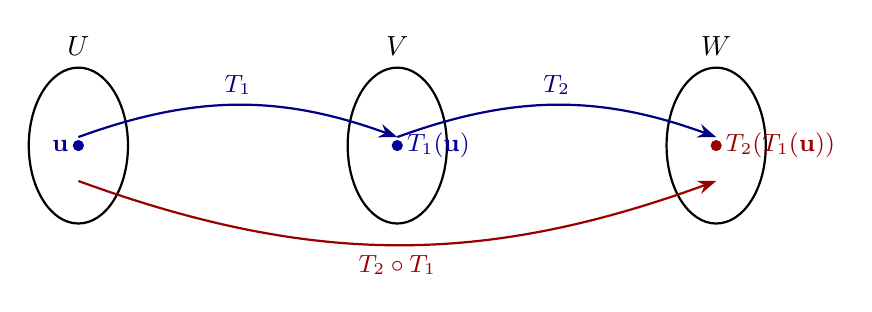
\begin{tikzpicture}[>=Stealth, scale=0.9]
  \draw[thick] (-4.5,0) ellipse (0.7 and 1.1);
  \node at (-4.5,1.4) {$U$};
  \draw[thick] (0,0) ellipse (0.7 and 1.1);
  \node at (0,1.4) {$V$};
  \draw[thick] (4.5,0) ellipse (0.7 and 1.1);
  \node at (4.5,1.4) {$W$};
  \filldraw[blue!60!black] (-4.5,0) circle (2pt) node[left, font=\small]{$\mathbf{u}$};
  \filldraw[blue!60!black] (0,0) circle (2pt) node[right, font=\small]{$T_1(\mathbf{u})$};
  \filldraw[red!60!black] (4.5,0) circle (2pt) node[right, font=\small]{$T_2(T_1(\mathbf{u}))$};
  \draw[->, thick, blue!50!black] (-4.5,0.12) to[out=20, in=160]
    node[above, font=\small]{$T_1$} (0,0.12);
  \draw[->, thick, blue!50!black] (0,0.12) to[out=20, in=160]
    node[above, font=\small]{$T_2$} (4.5,0.12);
  \draw[->, thick, red!60!black] (-4.5,-0.5) to[out=-20, in=-160]
    node[below, font=\small]{$T_2 \circ T_1$} (4.5,-0.5);
\end{tikzpicture}
\caption*{FIGURE 8.2.5\quad The composition $T_2 \circ T_1$.}
\end{figure}

\begin{tcolorbox}[colback=red!4, colframe=red!60!black,
  title={\textbf{Theorem 8.2.5}}, boxrule=0.5mm, arc=3mm]
If $T_1 : U \to V$ and $T_2 : V \to W$ are linear transformations, then $T_2 \circ T_1 : U \to W$
is also a linear transformation.
\end{tcolorbox}

\textbf{Proof.} For vectors $\mathbf{u},\mathbf{v}$ in $U$ and scalar $c$:
\begin{align*}
  (T_2\circ T_1)(\mathbf{u}+\mathbf{v})
    &= T_2(T_1(\mathbf{u}+\mathbf{v})) = T_2(T_1(\mathbf{u})+T_1(\mathbf{v}))\\
    &= T_2(T_1(\mathbf{u}))+T_2(T_1(\mathbf{v}))
     = (T_2\circ T_1)(\mathbf{u}) + (T_2\circ T_1)(\mathbf{v})\\[2pt]
  (T_2\circ T_1)(c\mathbf{u})
    &= T_2(T_1(c\mathbf{u})) = T_2(cT_1(\mathbf{u})) = cT_2(T_1(\mathbf{u}))
     = c(T_2\circ T_1)(\mathbf{u}) \quad\blacksquare
\end{align*}

\subsection*{EXAMPLE 10 | Composition of Linear Transformations}

Let $T_1 : P_1 \to P_2$ and $T_2 : P_2 \to P_2$ be given by
$T_1(p(x)) = xp(x)$ and $T_2(p(x)) = p(2x+4)$.
Then $(T_2 \circ T_1)(p(x)) = T_2(xp(x)) = (2x+4)p(2x+4)$.
For $p(x) = c_0 + c_1 x$:
\[
  (T_2\circ T_1)(c_0+c_1x) = (2x+4)(c_0+c_1(2x+4)) = c_0(2x+4)+c_1(2x+4)^2
\]

\subsection*{EXAMPLE 11 | Composition with the Identity Operator}

If $T : V \to V$ is any linear operator and $I : V \to V$ is the identity operator, then
for all $\mathbf{v}$ in $V$:
\[
  (T \circ I)(\mathbf{v}) = T(I(\mathbf{v})) = T(\mathbf{v})
  \qquad
  (I \circ T)(\mathbf{v}) = I(T(\mathbf{v})) = T(\mathbf{v})
\]
Thus $T \circ I$ and $I \circ T$ are both the same as $T$:
\begin{equation}
  T \circ I = T \qquad \text{and} \qquad I \circ T = T \tag{5}
\end{equation}

Compositions extend to three or more transformations. If $T_1 : U\to V$, $T_2 : V\to W$,
$T_3 : W \to Y$, then
\begin{equation}
  (T_3 \circ T_2 \circ T_1)(\mathbf{u}) = T_3(T_2(T_1(\mathbf{u}))) \tag{6}
\end{equation}

\begin{figure}[ht]
\centering
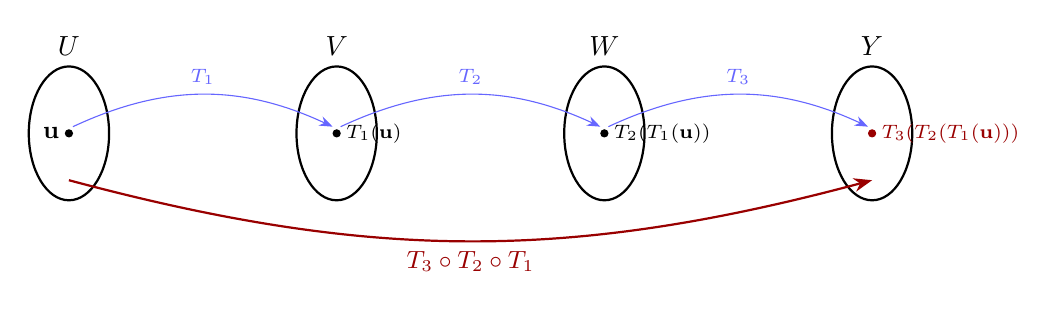
\begin{tikzpicture}[>=Stealth, scale=0.85]
  \foreach \x/\lbl in {-6/U, -2/V, 2/W, 6/Y}{
    \draw[thick] (\x,0) ellipse (0.6 and 1.0);
    \node at (\x,1.3) {$\lbl$};
  }
  \filldraw (-6,0) circle (1.5pt) node[left, font=\small]{$\mathbf{u}$};
  \filldraw (-2,0) circle (1.5pt) node[right, font=\scriptsize]{$T_1(\mathbf{u})$};
  \filldraw (2,0) circle (1.5pt) node[right, font=\scriptsize]{$T_2(T_1(\mathbf{u}))$};
  \filldraw[red!60!black] (6,0) circle (1.5pt) node[right, font=\scriptsize]{$T_3(T_2(T_1(\mathbf{u})))$};
  \draw[->, blue!60] (-5.94,0.1) to[out=25, in=155] node[above, font=\scriptsize]{$T_1$} (-2.06,0.1);
  \draw[->, blue!60] (-1.94,0.1) to[out=25, in=155] node[above, font=\scriptsize]{$T_2$} (1.94,0.1);
  \draw[->, blue!60] (2.06,0.1) to[out=25, in=155] node[above, font=\scriptsize]{$T_3$} (5.94,0.1);
  \draw[->, thick, red!60!black] (-6,-0.7) to[out=-15, in=-165]
    node[below, font=\small]{$T_3\circ T_2\circ T_1$} (6,-0.7);
\end{tikzpicture}
\caption*{FIGURE 8.2.6\quad Composition of three linear transformations.}
\end{figure}

\vspace{2mm}

\redheading{Composition of One-to-One Linear Transformations}

\begin{tcolorbox}[colback=red!4, colframe=red!60!black,
  title={\textbf{Theorem 8.2.6}}, boxrule=0.5mm, arc=3mm]
If $T_1 : U \to V$ and $T_2 : V \to W$ are one-to-one linear transformations, then:
\begin{enumerate}
  \item[(a)] $T_2 \circ T_1$ is one-to-one.
  \item[(b)] $(T_2 \circ T_1)^{-1} = T_1^{-1} \circ T_2^{-1}$.
\end{enumerate}
\end{tcolorbox}

\textbf{Proof of (a).} If $\mathbf{u}$ and $\mathbf{v}$ are distinct vectors in $U$, then
$T_1(\mathbf{u}) \neq T_1(\mathbf{v})$ (since $T_1$ is one-to-one), and then
$T_2(T_1(\mathbf{u})) \neq T_2(T_1(\mathbf{v}))$ (since $T_2$ is one-to-one).
So $(T_2\circ T_1)(\mathbf{u}) \neq (T_2\circ T_1)(\mathbf{v})$. $\blacksquare$

\medskip
\textbf{Proof of (b).} Let $\mathbf{u} = (T_2\circ T_1)^{-1}(\mathbf{w})$ for any $\mathbf{w}$
in the range of $T_2\circ T_1$. Then $(T_2\circ T_1)(\mathbf{u}) = \mathbf{w}$, i.e.,
$T_2(T_1(\mathbf{u})) = \mathbf{w}$. Taking $T_2^{-1}$ gives $T_1(\mathbf{u}) = T_2^{-1}(\mathbf{w})$,
and then taking $T_1^{-1}$ gives $\mathbf{u} = T_1^{-1}(T_2^{-1}(\mathbf{w})) =
(T_1^{-1}\circ T_2^{-1})(\mathbf{w})$. $\blacksquare$

Part (b) generalizes: the inverse of a composition is the composition of the inverses
in \emph{reverse} order. For three transformations:
\begin{equation}
  (T_3\circ T_2\circ T_1)^{-1} = T_1^{-1}\circ T_2^{-1}\circ T_3^{-1} \tag{8}
\end{equation}
For matrix transformations this gives $(T_{BA})^{-1} = T_{A^{-1}B^{-1}}$ and
$(T_{CBA})^{-1} = T_{A^{-1}B^{-1}C^{-1}}$, or equivalently:
\begin{equation}
  (BA)^{-1} = A^{-1}B^{-1} \qquad \text{and} \qquad (CBA)^{-1} = A^{-1}B^{-1}C^{-1} \tag{9}
\end{equation}

\vspace{3mm}
\noindent\rule{\linewidth}{0.5pt}

\section*{Exercise Set 8.2}

\noindent\textit{In Exercises 1--2, determine whether the stated matrix operator is one-to-one.}

\begin{enumerate}
  \item \textbf{a.} The orthogonal projection onto the $x$-axis in $R^2$.\\
        \textbf{b.} The reflection about the $y$-axis in $R^2$.\\
        \textbf{c.} The reflection about the line $y=x$ in $R^2$.

  \item[2.] \textbf{a.} A rotation about the $z$-axis in $R^3$.\\
        \textbf{b.} A reflection about the $xy$-plane in $R^3$.\\
        \textbf{c.} An orthogonal projection onto the $xz$-plane in $R^3$.

\end{enumerate}

\noindent\textit{In Exercises 3--4, determine whether $T$ is one-to-one by finding its kernel
and applying Theorem~8.2.1.}

\begin{enumerate}
  \item[3.] \textbf{a.} $T : R^2 \to R^2$, $T(x,y)=(y,x)$.\\
        \textbf{b.} $T : R^2 \to R^3$, $T(x,y)=(x,y,x+y)$.\\
        \textbf{c.} $T : R^3 \to R^2$, $T(x,y,z)=(x+y+z,\,x-y-z)$.

  \item[4.] \textbf{a.} $T : R^2 \to R^3$, $T(x,y)=(x-y,\,y-x,\,2x-2y)$.\\
        \textbf{b.} $T : R^2 \to R^2$, $T(x,y)=(0,2x+3y)$.\\
        \textbf{c.} $T : R^2 \to R^2$, $T(x,y)=(x+y,\,x-y)$.

\end{enumerate}

\noindent\textit{In Exercises 5--6, use Theorem~8.2.3 to determine whether $T_A$ is
one-to-one, onto, both, or neither.}

\begin{enumerate}
  \item[5.] \textbf{a.} $A = \begin{bmatrix}1&-2\\2&-4\\-3&6\end{bmatrix}$
        \quad \textbf{b.} $A = \begin{bmatrix}1&3&1&7\\2&7&2&4\\-1&-3&0&0\end{bmatrix}$

  \item[7.] Use the given information to determine whether $T$ is one-to-one.\\
        \textbf{a.} $T : V \to W$; $\text{nullity}(T) = 0$.\\
        \textbf{b.} $T : V \to W$; $\text{rank}(T) = \dim(V)$.\\
        \textbf{c.} $T : V \to W$; $\dim(W) < \dim(V)$.

  \item[8.] Use the given information to determine whether the linear operator $T : V \to V$
        is one-to-one, onto, both, or neither.\\
        \textbf{a.} $T : V \to V$; $\text{nullity}(T) = 0$.\\
        \textbf{b.} $T : V \to V$; $\text{rank}(T) < \dim(V)$.

  \item[11.] Let $\mathbf{a}$ be a fixed vector in $R^3$. Does $T(\mathbf{v}) = \mathbf{a}\times\mathbf{v}$
        define a one-to-one linear operator on $R^3$? Explain.

  \item[12.] Let $E$ be a fixed $2\times 2$ elementary matrix. Does $T(A) = EA$ define a
        one-to-one linear operator on $M_{22}$? Explain.

\end{enumerate}

\noindent\textit{In Exercises 13--14, use Theorem~8.2.3 to determine whether multiplication
by $A$ is one-to-one, onto, both, or neither.}

\begin{enumerate}
  \item[13.] \textbf{a.} $A = \begin{bmatrix}1&2\\3&5\end{bmatrix}$
        \quad \textbf{b.} $A = \begin{bmatrix}1&3&1&1\\1&4&0&0\end{bmatrix}$
        \quad \textbf{c.} $A = \begin{bmatrix}5&4\\1&1\end{bmatrix}$

  \item[15.] In words, describe the inverse of each operator.\\
        \textbf{a.} Reflection about the $x$-axis in $R^2$.\\
        \textbf{b.} Rotation about the origin through $\pi/4$ in $R^2$.

  \item[17.] Use matrix inversion to confirm the stated result in $R^2$.\\
        \textbf{a.} The inverse of a reflection about $y=x$ is a reflection about $y=x$.\\
        \textbf{b.} The inverse of a rotation through $\theta$ is a rotation through $-\theta$.

  \item[19.] Let $T : P_1 \to R^2$ be defined by $T(p(x)) = (p(0), p(1))$.\\
        \textbf{a.} Find $T(1-2x)$.\\
        \textbf{b.} Show $T$ is a linear transformation.\\
        \textbf{c.} Show $T$ is one-to-one.\\
        \textbf{d.} Find $T^{-1}(2,3)$ and sketch its graph.

  \item[20.] Determine whether $T : R^n \to R^n$ is one-to-one; if so, find $T^{-1}$.\\
        \textbf{a.} $T(x_1,\ldots,x_n) = (0,x_1,x_2,\ldots,x_{n-1})$.\\
        \textbf{b.} $T(x_1,x_2,\ldots,x_n) = (x_n,x_{n-1},\ldots,x_2,x_1)$.

\end{enumerate}

\noindent\textit{In Exercises 23--24, compute $(T_2 \circ T_1)(x,y)$.}

\begin{enumerate}
  \item[23.] $T_1(x,y) = (2x,3y)$, $T_2(x,y) = (x-y,\,x+y)$.

  \item[24.] $T_1(x,y) = (2x,-3y,x+y)$, $T_2(x,y,z) = (x-y,\,y+z)$.

  \item[25.] Let $T_1 : P_2 \to P_2$ and $T_2 : P_2 \to P_3$ be given by
        $T_1(p(x)) = p(x+1)$ and $T_2(p(x)) = xp(x)$.
        Find $(T_2\circ T_1)(a_0+a_1x+a_2x^2)$.

  \item[26.] Let $T_1 : P_n \to P_n$ and $T_2 : P_n \to P_n$ be defined by
        $T_1(p(x)) = p(x-1)$ and $T_2(p(x)) = p(x+1)$.
        Find $(T_1\circ T_2)(p(x))$ and $(T_2\circ T_1)(p(x))$.

  \item[27.] Let $T_1 : M_{22} \to R$ and $T_2 : M_{22} \to M_{22}$ be defined by
        $T_1(A) = \mathrm{tr}(A)$ and $T_2(A) = A^T$.\\
        \textbf{a.} Find $(T_1\circ T_2)(A)$ where $A = \begin{bmatrix}a&b\\c&d\end{bmatrix}$.\\
        \textbf{b.} Can you find $(T_2\circ T_1)(A)$? Explain.

  \item[32.] Let $T_1 : R^2 \to R^2$ and $T_2 : R^2 \to R^2$ be the operators
        $T_1(x,y)=(x+y,\,x-y)$ and $T_2(x,y)=(2x+y,\,x-2y)$.\\
        \textbf{a.} Show $T_1$ and $T_2$ are one-to-one.\\
        \textbf{b.} Find $T_1^{-1}(x,y)$, $T_2^{-1}(x,y)$, and $(T_2\circ T_1)^{-1}(x,y)$.\\
        \textbf{c.} Verify $(T_2\circ T_1)^{-1} = T_1^{-1}\circ T_2^{-1}$.

  \item[35.] Let $T : R^3 \to R^3$ be orthogonal projection onto the $xy$-plane.
        Show $T\circ T = T$.

  \item[38.] \textit{(Calculus required)} Let $D : P_n \to P_{n-1}$ by $D(p(x)) = p'(x)$
        and $J : P_{n-1} \to P_n$ by $J(p(x)) = \displaystyle\int_0^x p(t)\,dt$.\\
        \textbf{a.} Show $D$ and $J$ are linear.\\
        \textbf{b.} Explain why $J$ is not the inverse of $D$.\\
        \textbf{c.} Can the domains/codomains of $D$ and $J$ be restricted so they are
        inverse linear transformations?

\end{enumerate}

\noindent\textit{Working with Proofs}

\begin{enumerate}
  \item[44.] Prove: if there is an onto linear transformation $T : V \to W$, then
        $\dim(V) \geq \dim(W)$.

  \item[45.] Prove: if $T : V \to W$ is a one-to-one linear transformation, then
        $T^{-1} : R(T) \to V$ is also a one-to-one linear transformation.

  \item[46.] Using Formula~(6), prove:\\
        \textbf{a.} $T_3\circ T_2\circ T_1$ is a linear transformation.\\
        \textbf{b.} $T_3\circ T_2\circ T_1 = (T_3\circ T_2)\circ T_1$.\\
        \textbf{c.} $T_3\circ T_2\circ T_1 = T_3\circ(T_2\circ T_1)$.

  \item[47.] Let $V$ and $W$ be finite-dimensional and $T : V \to W$ linear. Prove:\\
        \textbf{a.} If $\dim(V) > \dim(W)$, then $T$ cannot be one-to-one.\\
        \textbf{b.} If $\dim(V) < \dim(W)$, then $T$ cannot be onto.

\end{enumerate}

\end{document}
